\chapter{Pokémon, Yo-kai Watch and the Global Yōkai}

\section{Character culture}

\begin{definition}[Kyara]
\emph{Kyara} (\ja{キャラ}, from English ``character'') are visual characters detached from
any single story, which circulate across goods, ads, games and media: Hello Kitty,
Kumamon, Pikachu. Japan's ``character business'' is enormous; local governments and even
police forces have mascot characters (\ja{ゆるキャラ}, yuru-kyara, ``loose/relaxed
characters'').
\end{definition}

The theme of the last week: the long history of yōkai cataloguing (Sekien, Mizuki) prepared
Japanese popular culture to treat monsters as \emph{collectible characters}. Pokémon and
Yo-kai Watch are the logical end point.

\begin{center}
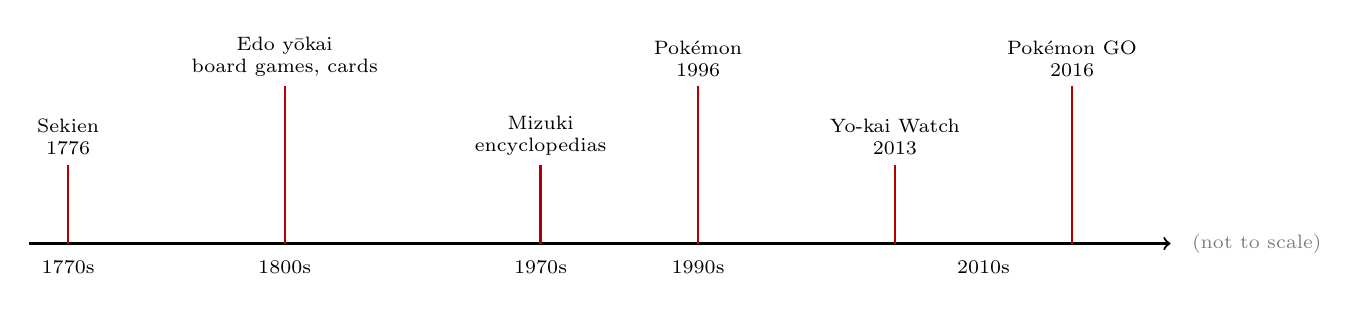
\begin{tikzpicture}[x=0.5cm, y=1cm, every node/.style={font=\scriptsize}]
  \draw[->, thick] (0,0) -- (29,0);
  \foreach \x/\h/\lab in {1/1.0/{Sekien\\1776}, 6.5/2.0/{Edo yōkai\\board games, cards}, 13/1.0/{Mizuki\\encyclopedias}, 17/2.0/{Pokémon\\1996}, 22/1.0/{Yo-kai Watch\\2013}, 26.5/2.0/{Pokémon GO\\2016}} {
    \draw[red!70!black, thick] (\x,0) -- (\x,\h);
    \node[above, align=center] at (\x,\h) {\lab};
  }
  \node[below] at (1,-0.1) {1770s};
  \node[below] at (6.5,-0.1) {1800s};
  \node[below] at (13,-0.1) {1970s};
  \node[below] at (17,-0.1) {1990s};
  \node[below] at (24.25,-0.1) {2010s};
  \node[gray, anchor=west] at (29.3,0) {(not to scale)};
\end{tikzpicture}
\end{center}

\section{Pokémon}

\subsection{Origins}

\textbf{Pokémon} (\ja{ポケモン}, from \emph{Pocket Monsters}) began as a pair of Game Boy games
(\emph{Red} and \emph{Green}, 1996) designed by \textbf{Tajiri Satoshi} of Game Freak, published
by Nintendo. Tajiri grew up collecting insects in the suburbs of Tokyo (Machida) as they
were being developed and wanted children to experience the joy of catching and collecting
creatures. A trading card game (1996), anime (1997) and films followed; the franchise is the
highest-grossing media franchise in the world.

\subsection{The game logic}

\begin{itemize}
  \item \textbf{Catch}: throw a Poké Ball to capture a wild monster.
  \item \textbf{Collect}: fill the \textbf{Pokédex}, an encyclopedia with an entry for
        each species (``Gotta catch 'em all!'').
  \item \textbf{Battle and train}: Pokémon fight other trainers' Pokémon; they gain
        experience and \textbf{evolve} into new forms.
  \item \textbf{Trade}: two versions of the game have different species, so players must
        trade via cable link: sociality built into the design.
\end{itemize}

\begin{important}[Pokémon as a descendant of the yōkai catalogue]
\begin{itemize}
  \item The Pokédex is formally like Sekien's catalogues: one creature per entry, a picture,
        a name, a short descriptive text (Week 5).
  \item Many Pokémon are based on yōkai and folklore: Ninetales (nine-tailed fox), Vulpix
        (kitsune), Ludicolo (kappa-like, with a dish-like lily pad on its head), Shiftry
        (tengu: long nose, leaf fans), Froslass (yuki-onna), Banette (an abandoned doll,
        a tsukumogami) and Gengar (often compared to shadowy yōkai).
  \item But Pokémon are also derived from \emph{insect collecting} and \emph{natural history}:
        the trainer is a field naturalist, Professor Oak a museum curator.
\end{itemize}
\end{important}

\begin{example}[Taming the monster]
In yōkai lore, a monster is controlled by a ritual specialist (an onmyōji binds shikigami,
Week 4). In Pokémon, every child becomes such a specialist: wild monsters are caught,
named, carried in a ball and made to fight on your behalf. Anne Allison (\emph{Millennial
Monsters}, 2006) calls this ``pocketability'': monsters become portable companions that
soothe the isolation of busy, mobile, post-bubble Japanese life.
\end{example}

\subsection{Pokémon goes global}

\begin{itemize}
  \item 1998--99: Pokémon arrived in North America (the anime was edited: rice balls
        renamed ``jelly-filled donuts'', Japanese text removed). ``Pokémania'' followed:
        cards were banned in some schools, and there were moral panics in the US about
        gambling and occult influence.
  \item The ``culturally odourless'' debate (Iwabuchi; see EASIA 201R, Week 12): Pokémon
        travelled as a global product with its Japaneseness muted, yet its creature-logic
        is deeply rooted in Japanese traditions.
  \item \textbf{Pokémon GO} (2016): an augmented-reality smartphone game in which players
        catch Pokémon in real locations, overlaying a monster world onto the physical one, a
        digital hyakki yagyō. Shrines and temples became ``PokéStops'' (some asked to be
        removed).
\end{itemize}

\section{Yo-kai Watch}

\textbf{Yo-kai Watch} (\ja{妖怪ウォッチ}) began as a Nintendo 3DS game by Level-5 (2013),
followed by an anime (2014), toys and films. It was a massive hit in Japan and set off the
latest ``yōkai boom''.

\begin{itemize}
  \item The boy \textbf{Keita} (Nate in English) receives a watch that lets him see yōkai.
        His companion is \textbf{Whisper}, a ghost butler, and his favourite yōkai is the
        cat \textbf{Jibanyan}, the spirit of a cat killed by a truck (a jibakurei, a ghost
        bound to its place of death, made cute).
  \item The central idea: everyday annoyances (forgetting things, arguing, being lazy,
        craving snacks) are caused by yōkai possessing people. Yōkai explain the
        inexplicable, exactly as in Foster's definition (Week 1), but the mysteries are
        trivial and comic.
  \item Players befriend yōkai and receive \textbf{medals} to summon them; the
        \textbf{Yo-kai Medallium} is the in-game encyclopedia. Toy watches and medals sold
        in the millions.
  \item Many Yo-kai Watch characters are puns (Jibanyan = jibakurei + nyan, the cat's
        meow), in the tradition of Sekien's wordplay.
\end{itemize}

\begin{center}
\begin{tabular}{p{3.2cm}p{4.8cm}p{4.8cm}}
\toprule
 & Pokémon (1996) & Yo-kai Watch (2013) \\
\midrule
Creatures called & ``pocket monsters'' & yōkai (explicitly) \\
Origin of creatures & animals, insects, objects, some folklore & folklore, puns, everyday life \\
Relationship & catch, train, battle & befriend, summon \\
Encyclopedia & Pokédex & Yo-kai Medallium \\
Setting & invented world & ordinary Japanese suburb \\
Global reach & enormous & strong in Japan; limited abroad \\
\bottomrule
\end{tabular}
\end{center}

\section{The global yōkai}

Japanese monsters now circulate around the world through manga, anime, games and film:

\begin{itemize}
  \item Manga/anime with yōkai themes: \emph{Inuyasha} (half-dog demon), \emph{Natsume's
        Book of Friends}, \emph{Mushishi}, \emph{Naruto} (tailed beasts), \emph{Demon
        Slayer} (oni).
  \item Video games: \emph{Ōkami} (the sun goddess Amaterasu as a wolf, Orochi as a boss),
        \emph{Nioh}, \emph{Ghost of Tsushima}.
  \item Hollywood: \emph{Pacific Rim} (2013) took the word ``kaijū'' into English; Legendary
        Pictures' MonsterVerse; \emph{Detective Pikachu} (2019).
  \item Foster's \emph{Book of Yōkai} (2015) and online databases (e.g.\ the
        International Research Center for Japanese Studies' yōkai image database) make
        yōkai a subject of global study.
\end{itemize}

\begin{center}
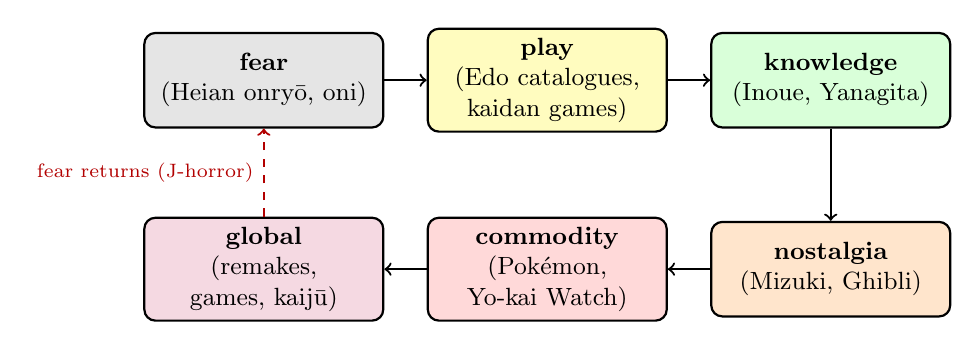
\begin{tikzpicture}[b/.style={draw, thick, rounded corners, align=center, font=\small, text width=2.8cm, minimum height=1.2cm}]
  \node[b, fill=gray!20] (fear) at (0,0) {\textbf{fear}\\(Heian onryō, oni)};
  \node[b, fill=yellow!25] (play) at (3.6,0) {\textbf{play}\\(Edo catalogues, kaidan games)};
  \node[b, fill=green!15] (know) at (7.2,0) {\textbf{knowledge}\\(Inoue, Yanagita)};
  \node[b, fill=orange!20] (nost) at (7.2,-2.4) {\textbf{nostalgia}\\(Mizuki, Ghibli)};
  \node[b, fill=red!15] (comm) at (3.6,-2.4) {\textbf{commodity}\\(Pokémon, Yo-kai Watch)};
  \node[b, fill=purple!15] (glob) at (0,-2.4) {\textbf{global}\\(remakes, games, kaijū)};
  \draw[->, thick] (fear) -- (play); \draw[->, thick] (play) -- (know);
  \draw[->, thick] (know) -- (nost); \draw[->, thick] (nost) -- (comm);
  \draw[->, thick] (comm) -- (glob);
  \draw[->, thick, dashed, red!70!black] (glob) -- node[left, font=\scriptsize] {fear returns (J-horror)} (fear);
\end{tikzpicture}
\end{center}

\begin{important}[Final essay themes (as discussed in the last lecture)]
\begin{enumerate}
  \item Choose one creature and trace its transformation across at least three periods
        and media (e.g.\ the kitsune from Inari to Tamamo no Mae to Ninetales).
  \item ``Monsters are never just monsters'': analyse one film or text as a response to
        its historical moment (Godzilla and 1954; Sadako and the 1990s).
  \item Is the commodification of yōkai the death of folklore, or its newest form?
\end{enumerate}
\end{important}

\begin{aside}
The professor ended with Cohen's seventh thesis: monsters ask us why we created them. My
note in the margin: ``Japan created monsters to explain disasters, then to have fun, then
to sell things, and at every stage the monsters also kept telling people something about
themselves.''
\end{aside}

\section*{Summary}
\begin{itemize}
  \item Character (kyara) culture treats monsters as collectible, portable figures.
  \item Pokémon (1996): catch, collect (Pokédex), battle, evolve, trade; descends from
        Sekien's catalogues and insect collecting; global phenomenon.
  \item Yo-kai Watch (2013): yōkai as causes of everyday annoyances; befriend and summon;
        pun-based design.
  \item Yōkai have moved from fear to play, knowledge, nostalgia, commodity and global
        circulation, while fear keeps returning.
\end{itemize}
